\section{Durchführung}
\label{sec:Durchführung}
Die Durchführung gliedert sich in zwei Teile, zum einen die Messung
des brechenden Winkels $\varphi$ des Prismas, zum anderen die Messung
der Beugungswinkel $\eta$ der Spektrallinien.

\subsection{a}%$\varphi$-Messung}
Für diese Messung wird das Prisma so in den Strahlengang gebracht, dass
das Licht parallel auf die Spitze der brechenden Kanten fällt.
Dabei wird das Licht von den Prismenoberflächen reflektiert.
Dieser Aufbau ist in Abbildung \ref{fig:phi} zu sehen.

\begin{figure}[H]
  \centering
  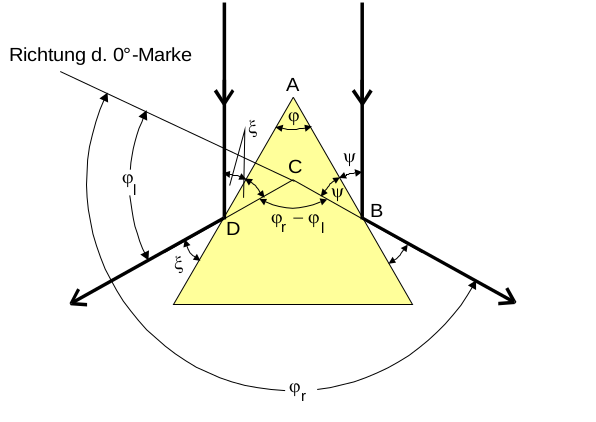
\includegraphics[height=5cm]{dreh.png}
  \caption{Bestimmung des Winkels zwischen den brechenden Kanten.}
  \label{fig:phi}
  \cite{skript}
\end{figure}

Es werden 7 verschiedene Wertepaare von $\varphi_r$ und $\varphi_l$,
den Winkeln unter denen der reflektierte Strahl zu beobachten ist
gemessen. Dazu wird die Position des Prismas vor jeder Messung leicht
verändert.
Der gesuchte Wilkel $\varphi$ ergibt sich durch
\begin{equation}
  \varphi=\frac{1}{2}(\varphi_r-\varphi_l).
  \label{eqn:phi}
\end{equation}

Der Versuchsaufbau, sowie die Messapparatur sind in Abbildung
\ref{fig:aufbau} zu sehen.

\begin{figure}
  \centering
  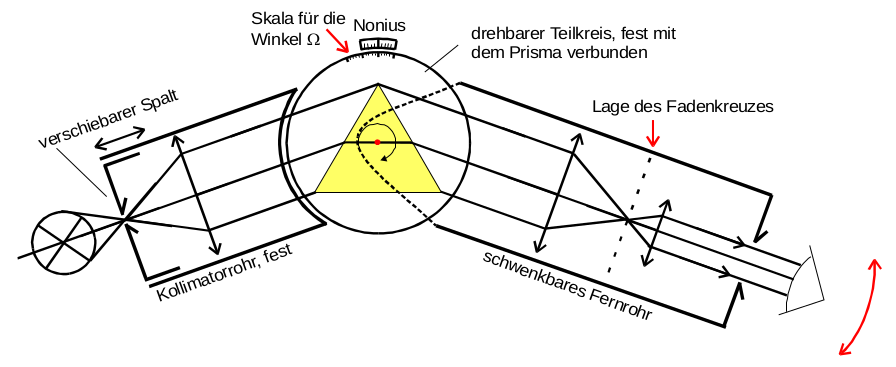
\includegraphics[width=11cm]{aufbau.png}
  \caption{Aufbau und Messapparatur.}
  \label{fig:aufbau}
  \cite{skript}
\end{figure}

\subsection{a}%$\eta$-Messung}
Um die Beugungswinkel $\eta$ der Spektrallinien zu messen muss ein
paralleler Strahlengang vorliegen. Dazu muss der reflektierte
Strahl mit einer Spektralline übereinstimmen. Ist die Messapparatur
so eingestellt, dass das Fadenkreuz, der reflektierte Strahl und die
Spektrallinie übereinander liegen, wird der Winkel abgelesen.
Diese Messung wird für alle Spektrallinien vorgenommen.
Nachdem das Prisma gedreht wurde wird die Messung mit eienr
spiegelsymmetrischen Anordnung, wie in Abbildung
\ref{fig:spiegel}, wiederholt.

\begin{figure}[H]
  \centering
  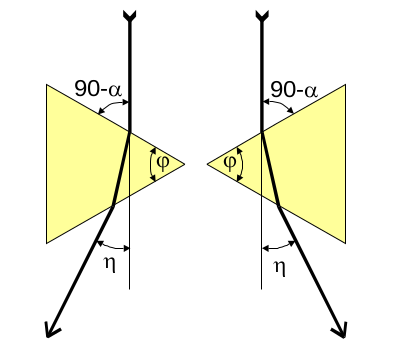
\includegraphics[height=5cm]{spiegel.png}
  \caption{Spiegelsymmetrische Anordnung zur Bestimmung des Brechungswinkels.}
  \label{fig:spiegel}
  \cite{skript}
\end{figure}

Aus den Wertepaaren $\eta_r$ und $\eta_l$ ergibt sich der gesucht
Brechungswinkel durch:
\begin{equation}
  \eta=180-(\eta_r - \eta_l).
  \label{eqn:eta}
\end{equation}

Der Brechungsindex kann aus $\varphi$ und $\eta$ mit der Formel
\begin{equation}
  n=\frac{\sin{(\frac{\eta+\varphi}{2})}}{\sin{(\frac{\varphi}{2})}}
  \label{eqn:brechungsindex}
\end{equation}
berechnet werden.
